\documentclass{article}
\usepackage{tikz}
\usepackage{fancybox}
\usetikzlibrary{shapes}

\usetikzlibrary{arrows}
\tikzset{
	treenode/.style = {align=center, inner sep=0pt, text centered,
		font=\sffamily},
	arn_n/.style = {treenode, circle, white, font=\sffamily\bfseries, draw=black,
		fill=black, text width=1.5em},% arbre rouge noir, noeud noir
	arn_r/.style = {treenode, circle, red, draw=red, 
		text width=1.5em, very thick},% arbre rouge noir, noeud rouge
	arn_x/.style = {treenode, rectangle, draw=black,
		minimum width=0.5em, minimum height=0.5em}% arbre rouge noir, nil
}


\usepackage{fancyvrb}  % for the Verbatim environment
\usepackage{graphicx}  % to include graphics
\usepackage{hyperref}  % for hyperlinks

\title{CS200 Functional Data Structures\\Assignment 4}
\author{Beep Beep: Affan-am00634 and Affan-sa00310}


\begin{document}
\maketitle
\section*{Problem 1. Meldable Heap}
	Please see the ass4.hs file in the same folder.
\section*{Problem 2. Heap Sort}
	Please see the ass4.hs file in the same folder.
\section*{Problem 3. Heap Operations}
	
\begin{enumerate}
	\item \textbf{10.1}
		Adding 7 to the BinaryHeap. 
		
		
		\begin{center}
			
			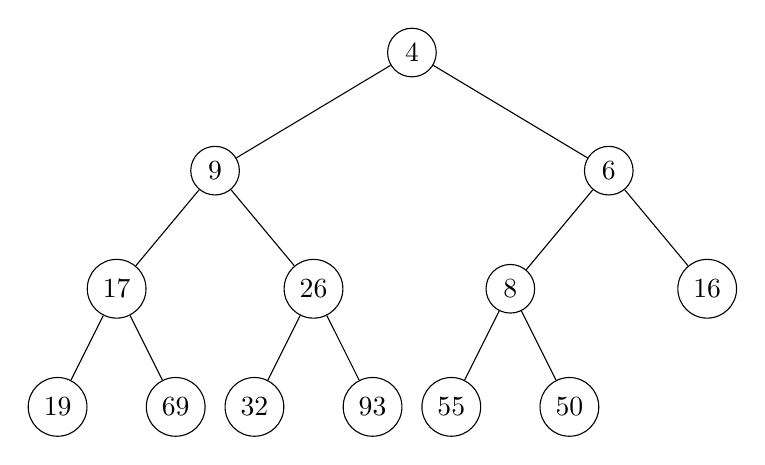
\begin{tikzpicture}[every node/.style={circle,draw},level 1/.style={sibling distance=50mm},level 2/.style={sibling distance=25mm},
			level 3/.style={sibling distance=15mm}
			]
			\node[circle,draw](z){4}
			child{
				node[circle, draw]{9} child{node[circle,draw] {17} child{node[circle,draw] {19}} child{node[circle,draw] {69}}} child{node[circle,draw] {26}
					child{node[circle,draw] {32}} child{node[circle,draw] {93}}
				}}
				child{
					node[circle,draw]{6} child{node[circle,draw] {8} child{node[circle,draw] {55} }
						child{node[circle,draw] {50} }
					} child{node[circle,draw] {16}} };
				\end{tikzpicture}
				
				\begin{tabular}{ |c|c|c|c|c|c|c|c|c|c|c|c|c|c|c| } 
					
					\hline
					4 & 9 & 6 & 17 & 26 & 8 & 16 & 19 & 69 & 32 & 93 & 55 & 50 & & \\
					\hline
					
				\end{tabular}
			\end{center}
			
			
			
			
			\begin{center}
				
				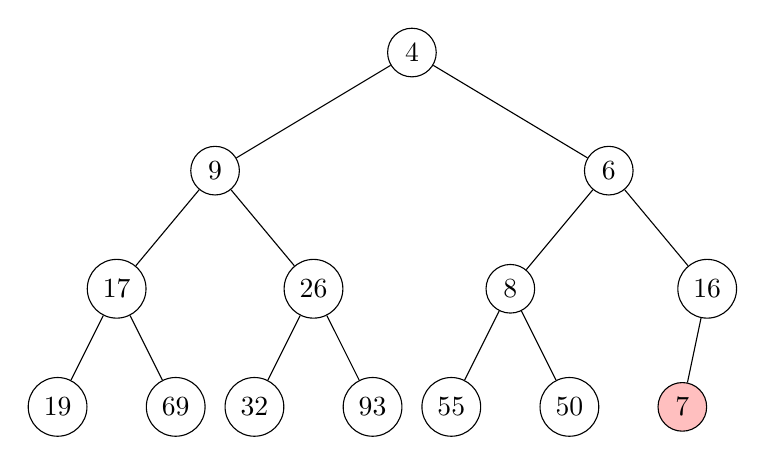
\begin{tikzpicture}[every node/.style={circle,draw},level 1/.style={sibling distance=50mm},level 2/.style={sibling distance=25mm},
				level 3/.style={sibling distance=15mm}
				]
				\node[circle,draw](z){4}
				child{
					node[circle, draw]{9} child{node[circle,draw] {17} child{node[circle,draw] {19}} child{node[circle,draw] {69}}} child{node[circle,draw] {26}
						child{node[circle,draw] {32}} child{node[circle,draw] {93}}
					}}
					child{
						node[circle,draw]{6} child{node[circle,draw] {8} child{node[circle,draw] {55} }
							child{node[circle,draw] {50} }
						}  child{node[circle,draw] {16} child{node[circle,draw,left,fill=pink]{7}}} 
					};
					\end{tikzpicture}
					
					\begin{tabular}{ |c|c|c|c|c|c|c|c|c|c|c|c|c|c|c| } 
						
						\hline
						4 & 9 & 6 & 17 & 26 & 8 & 16 & 19 & 69 & 32 & 93 & 55 & 50 & 7 & \\
						\hline
						
					\end{tabular}
				\end{center}
				
				\pagebreak
				
				Bubble up. 
				
				\begin{center}
					
					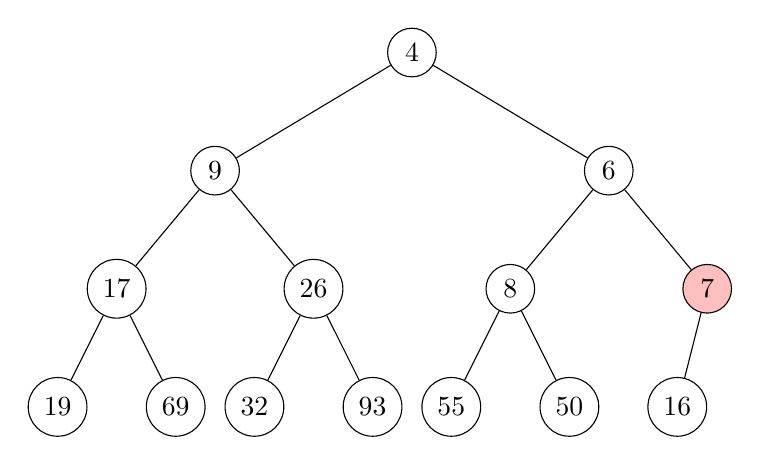
\begin{tikzpicture}[every node/.style={circle,draw},level 1/.style={sibling distance=50mm},level 2/.style={sibling distance=25mm},
					level 3/.style={sibling distance=15mm}
					]
					\node[circle,draw](z){4}
					child{
						node[circle, draw]{9} child{node[circle,draw] {17} child{node[circle,draw] {19}} child{node[circle,draw] {69}}} child{node[circle,draw] {26}
							child{node[circle,draw] {32}} child{node[circle,draw] {93}}
						}}
						child{
							node[circle,draw]{6} child{node[circle,draw] {8} child{node[circle,draw] {55} }
								child{node[circle,draw] {50} }
							}  child{node[circle,draw,fill=pink] {7} child{node[circle,draw,left]{16}}} 
						};
						\end{tikzpicture}
						
						\begin{tabular}{ |c|c|c|c|c|c|c|c|c|c|c|c|c|c|c| } 
							
							\hline
							4 & 9 & 6 & 17 & 26 & 8 & 7 & 19 & 69 & 32 & 93 & 55 & 50 & 16 & \\
							\hline
							
						\end{tabular}
					\end{center}
					
					Adding 3 to the BinaryHeap
					
					\begin{center}
						
						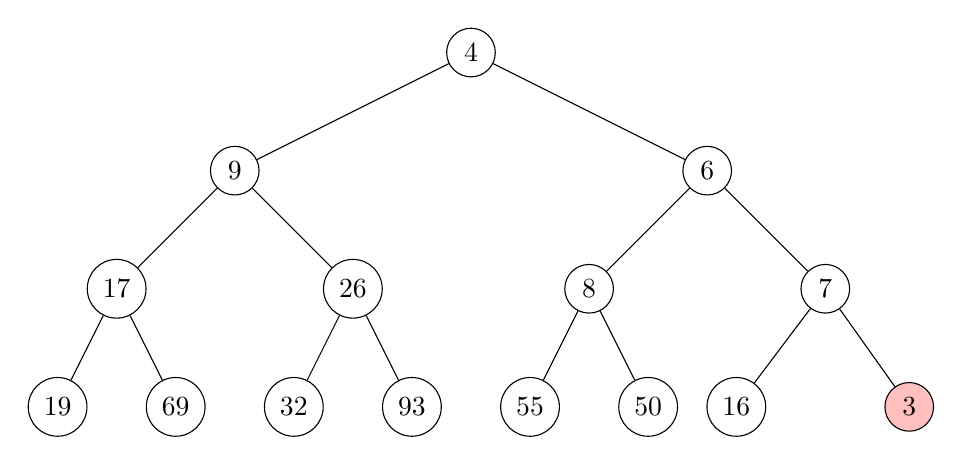
\begin{tikzpicture}[every node/.style={circle,draw},level 1/.style={sibling distance=60mm},level 2/.style={sibling distance=30mm},
						level 3/.style={sibling distance=15mm}
						]
						\node[circle,draw](z){4}
						child{
							node[circle, draw]{9} child{node[circle,draw] {17} child{node[circle,draw] {19}} child{node[circle,draw] {69}}} child{node[circle,draw] {26}
								child{node[circle,draw] {32}} child{node[circle,draw] {93}}
							}}
							child{
								node[circle,draw]{6} child{node[circle,draw] {8} child{node[circle,draw] {55} }
									child{node[circle,draw] {50} }
								}  child{node[circle,draw] {7} child{node[circle,draw,left]{16}}
								child{node[circle,draw,right,fill=pink]{3}} 
							}
						};
						\end{tikzpicture}
						
						\begin{tabular}{ |c|c|c|c|c|c|c|c|c|c|c|c|c|c|c| } 
							
							\hline
							4 & 9 & 6 & 17 & 26 & 8 & 7 & 19 & 69 & 32 & 93 & 55 & 50 & 16 & 3 \\
							\hline
								
						\end{tabular}
					\end{center}
					
					Bubble up 
					
					\begin{center}
						
						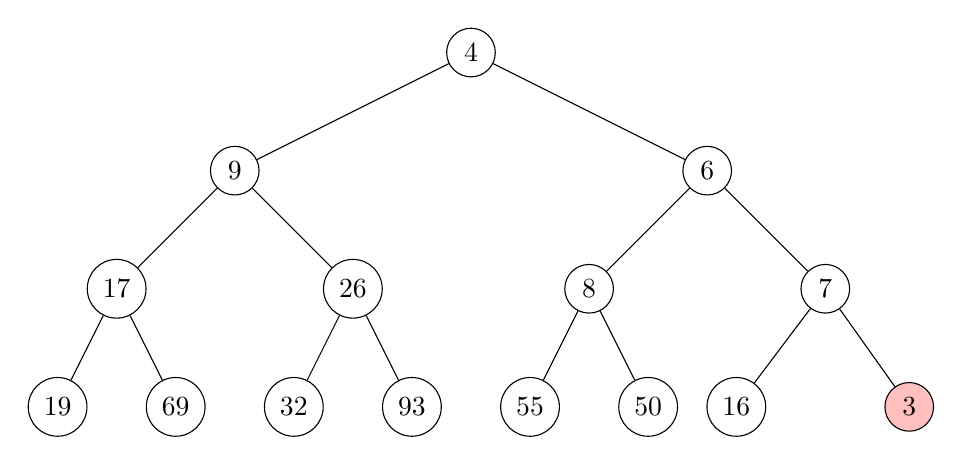
\begin{tikzpicture}[every node/.style={circle,draw},level 1/.style={sibling distance=60mm},level 2/.style={sibling distance=30mm},
						level 3/.style={sibling distance=15mm}
						]
						\node[circle,draw](z){4}
						child{
							node[circle, draw]{9} child{node[circle,draw] {17} child{node[circle,draw] {19}} child{node[circle,draw] {69}}} child{node[circle,draw] {26}
								child{node[circle,draw] {32}} child{node[circle,draw] {93}}
							}}
							child{
								node[circle,draw]{6} child{node[circle,draw] {8} child{node[circle,draw] {55} }
									child{node[circle,draw] {50} }
								}  child{node[circle,draw] {7} child{node[circle,draw,left]{16}}
								child{node[circle,draw,right, fill=pink]{3}} 
							}
						};
						\end{tikzpicture}
						
						\begin{tabular}{ |c|c|c|c|c|c|c|c|c|c|c|c|c|c|c| } 
							
							\hline
							4 & 9 & 6 & 17 & 26 & 8 & 3 & 19 & 69 & 32 & 93 & 55 & 50 & 16 & 7 \\
							\hline
							
						\end{tabular}
					\end{center}
					
					\begin{center}
						
						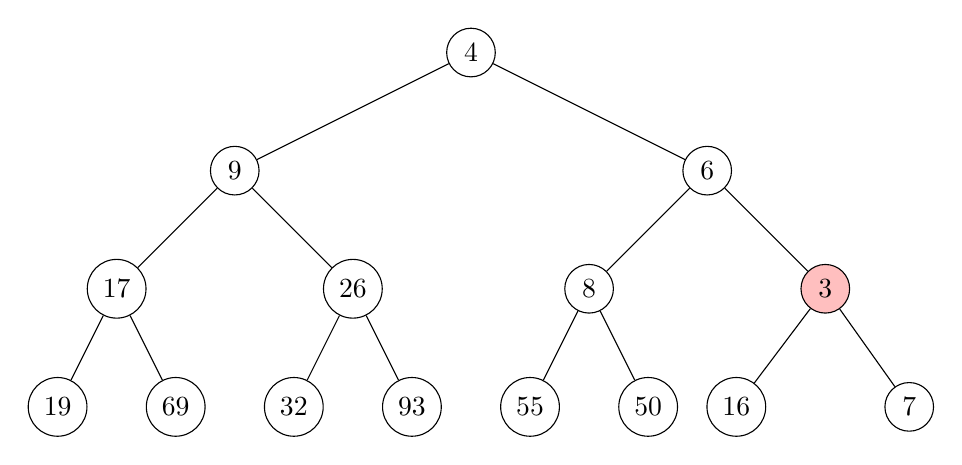
\begin{tikzpicture}[every node/.style={circle,draw},level 1/.style={sibling distance=60mm},level 2/.style={sibling distance=30mm},
						level 3/.style={sibling distance=15mm}
						]
						\node[circle,draw](z){4}
						child{
							node[circle, draw]{9} child{node[circle,draw] {17} child{node[circle,draw] {19}} child{node[circle,draw] {69}}} child{node[circle,draw] {26}
								child{node[circle,draw] {32}} child{node[circle,draw] {93}}
							}}
							child{
								node[circle,draw]{6} child{node[circle,draw] {8} child{node[circle,draw] {55} }
									child{node[circle,draw] {50} }
								}  child{node[circle,draw, fill=pink] {3} child{node[circle,draw,left]{16}}
								child{node[circle,draw,right]{7}} 
							}
						};
						\end{tikzpicture}
						
						\begin{tabular}{ |c|c|c|c|c|c|c|c|c|c|c|c|c|c|c| } 
							
							\hline
							4 & 9 & 3 & 17 & 26 & 8 & 6 & 19 & 69 & 32 & 93 & 55 & 50 & 16 & 7 \\
							\hline
							
							
						\end{tabular}
					\end{center}
					
					\begin{center}
						
						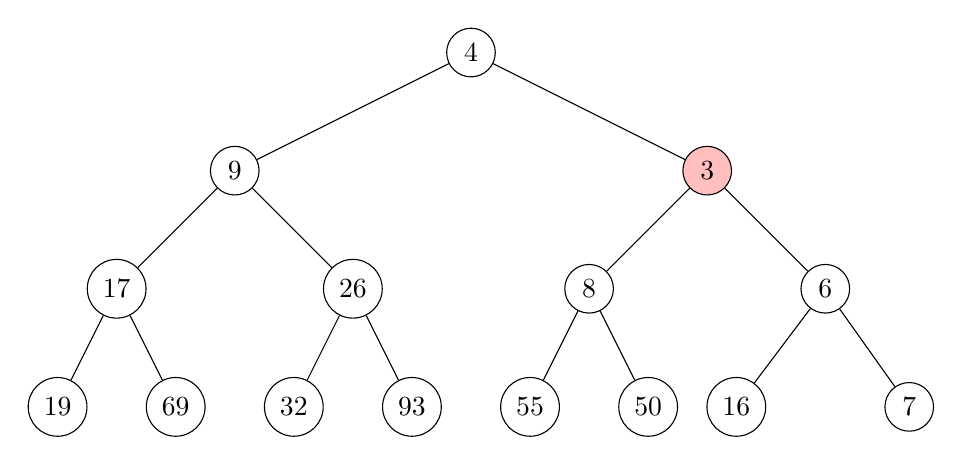
\begin{tikzpicture}[every node/.style={circle,draw},level 1/.style={sibling distance=60mm},level 2/.style={sibling distance=30mm},
						level 3/.style={sibling distance=15mm}
						]
						\node[circle,draw](z){4}
						child{
							node[circle, draw]{9} child{node[circle,draw] {17} child{node[circle,draw] {19}} child{node[circle,draw] {69}}} child{node[circle,draw] {26}
								child{node[circle,draw] {32}} child{node[circle,draw] {93}}
							}}
							child{
								node[circle,draw, fill=pink]{3} child{node[circle,draw] {8} child{node[circle,draw] {55} }
									child{node[circle,draw] {50} }
								}  child{node[circle,draw] {6} child{node[circle,draw,left]{16}}
								child{node[circle,draw,right]{7}} 
							}
						};
						\end{tikzpicture}
						
						\begin{tabular}{ |c|c|c|c|c|c|c|c|c|c|c|c|c|c|c| } 
							
							\hline
							3 & 9 & 4 & 17 & 26 & 8 & 6 & 19 & 69 & 32 & 93 & 55 & 50 & 16 & 7 \\
							\hline
								
						\end{tabular}
					\end{center}
					
					\begin{center}
						
						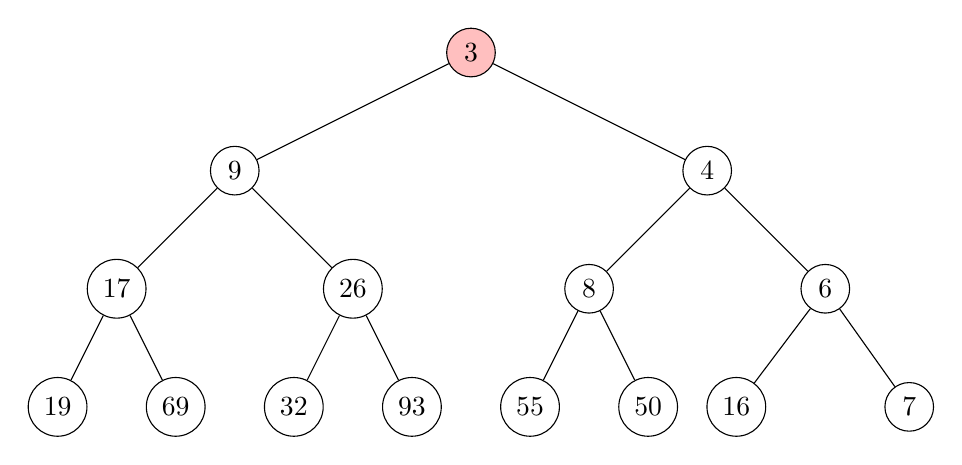
\begin{tikzpicture}[every node/.style={circle,draw},level 1/.style={sibling distance=60mm},level 2/.style={sibling distance=30mm},
						level 3/.style={sibling distance=15mm}
						]
						\node[circle,draw, fill=pink](z){3}
						child{
							node[circle, draw]{9} child{node[circle,draw] {17} child{node[circle,draw] {19}} child{node[circle,draw] {69}}} child{node[circle,draw] {26}
								child{node[circle,draw] {32}} child{node[circle,draw] {93}}
							}}
							child{
								node[circle,draw]{4} child{node[circle,draw] {8} child{node[circle,draw] {55} }
									child{node[circle,draw] {50} }
								}  child{node[circle,draw] {6} child{node[circle,draw,left]{16}}
								child{node[circle,draw,right]{7}} 
							}
						};
						\end{tikzpicture}
						
						\begin{tabular}{ |c|c|c|c|c|c|c|c|c|c|c|c|c|c|c| } 
							
						
						\hline
						3 & 9 & 4 & 17 & 26 & 8 & 6 & 19 & 69 & 32 & 93 & 55 & 50 & 16 & 7 \\
						\hline
							
						\end{tabular}
					\end{center}
					
	\item \textbf{10.7}
	\begin{enumerate}
		\item We begin with the tree provided:
		\begin{center}
		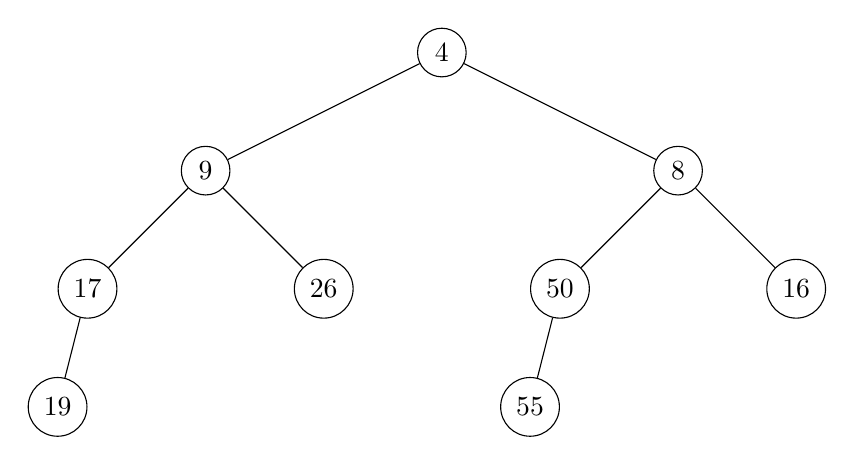
\begin{tikzpicture}[level/.style={sibling distance=60mm/#1}]
		\node[circle,draw] {4}
		 child{node[circle,draw] {9}
			 	  child{node[circle,draw] {17}
				 	  	child{node[circle,draw,left] {19}}
				 	  	}
				  child{node[circle,draw] {26}
					  	}
		 	  }
		 child{node[circle,draw] {8}
		 	child{node[circle,draw]{50}
		 		child{node[circle,draw,left]{55}}
			 	}
		 	child{node[circle,draw]{16}
			 	}
			 }
		; 
		\end{tikzpicture}
		\end{center}

		\item Remove the first item, we get the two following trees:
		\begin{center}
			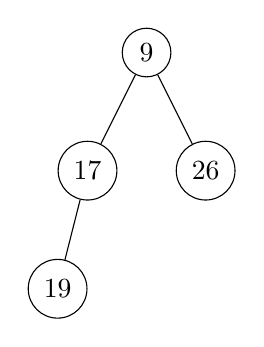
\begin{tikzpicture}
			
			\node[circle,draw] {9}
				child{node[circle,draw] {17}
					child{node[circle,draw,left] {19}}
				}
				child{node[circle,draw] {26}
				};
			\end{tikzpicture}
			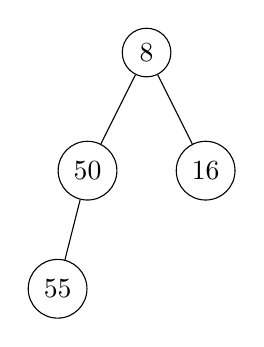
\begin{tikzpicture}
			\node[circle,draw] {8}
				child{node[circle,draw]{50}
					child{node[circle,draw,left]{55}}
				}
				child{node[circle,draw]{16}
				}
			; 
			\end{tikzpicture}
		\end{center}
		\item We merge the two trees merge(h1.right,h1.left). The algorithm takes care of the cases where node value x1>x2, therefore, we are not showing the swaps in our diagrams.
		\begin{center}
			\begin{tikzpicture}
			\node[circle,draw] {8}
			child{node[circle,draw]{50}
				child{node[circle,draw,left]{55}}
				}
			child{node[rectangle,draw,right]{
						\begin{tikzpicture}
						\node[circle,draw](a) {9}
						child{node[circle,draw] {17}
							child{node[circle,draw,left] {19}}
						}
						child{node[circle,draw] {26}
						}
						node[circle,draw, right of=a]{16}
						;\end{tikzpicture}
					}
			}
			;\end{tikzpicture}
		
			\end{center}
		\item Next recursive call, we do a coin flip for the node 9, because it is less than 16. We imagine that we get right on the random coin flip.
		\begin{center}
				\begin{tikzpicture}
				\node[circle,draw,level distance = 30mm] {8}
				child{node[circle,draw]{50}
					child{node[circle,draw,left]{55}}
				}
				child{node[rectangle,draw,right]{
							\begin{tikzpicture}
							\node[circle,draw,left](a) {9}
							child{node[circle,draw] {17}
								child{node[circle,draw,left] {19}}
							}
							child{node[rectangle,draw,right] {
										\begin{tikzpicture}
										\node[circle,draw](b){26}
										node[circle,draw,right of = b]{16}
										;\end{tikzpicture}
								}
							}
							;\end{tikzpicture}
					}
				}
				;\end{tikzpicture}
		\end{center}
		\item In the next recursive call, 16 is less than 26, therefore the resulting tree becomes;
			\begin{center}
				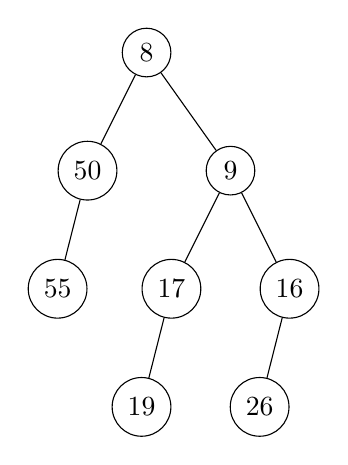
\begin{tikzpicture}
				\node[circle,draw] {8}
				child{node[circle,draw]{50}
					child{node[circle,draw,left]{55}}
				}
				child{node[circle,draw,right]{9}
						child{node[circle,draw] {17}
							child{node[circle,draw,left] {19}}
						}
						child{node[circle,draw]{16}
							child{node[circle,draw,left]{26}}
						}
				}
			;\end{tikzpicture}
		\end{center}
	\item Remove(8). First merge call would call merge on 8.left and 8.right
		\begin{center}
			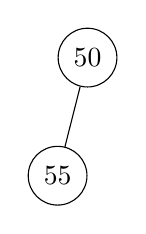
\begin{tikzpicture}
			\node[circle,draw] {50}
			child{node[circle,draw,left]{55}
			}
			;\end{tikzpicture}
			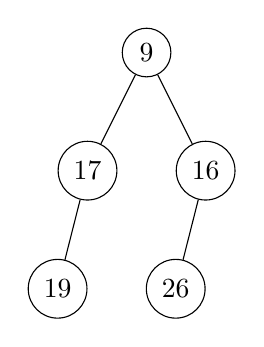
\begin{tikzpicture}
			\node[circle,draw,right]{9}
				child{node[circle,draw] {17}
					child{node[circle,draw,left] {19}}
				}
				child{node[circle,draw]{16}
					child{node[circle,draw,left]{26}}
				}
			;\end{tikzpicture}
		\end{center}
		
	\item Since 9 is less than 50, we would swap and then call the recursive function on a random child of 9 and the other tree. We assume we get random 1, and therefore, merge on the right child of 9.
	
	
	\begin{center}
		\begin{tikzpicture}
		\node[circle,draw]{9}
		child{node[circle,draw] {17}
			child{node[circle,draw,left] {19}}
		}
		child{node[rectangle,draw]{
				\begin{tikzpicture}
				\node[circle,draw](a) {50}
				child{node[circle,draw,left]{55}
				}
				node[circle,draw,left,right of = a]{16}
				child{node[circle,draw,left]{26}}
				;\end{tikzpicture}
			}
		}
		;\end{tikzpicture}
	\end{center}
	
	
	\item Next recursive call. We assume random to be 1 and therefore call is merge (16.right,h2) where h2 is the tree with node 50.
	
	
	\begin{center}
		\begin{tikzpicture}[level 1/.style={sibling distance=40mm, level distance = 20mm},
		level 2/.style={sibling distance=10mm, level distance = 10mm}]
		\node[circle,draw]{9}
		child{node[circle,draw] {17}
			child{node[circle,draw,left] {19}}
		}
		child{node[rectangle,draw]{
				\begin{tikzpicture}
				\node[circle,draw,left]{16}
				child{node[circle,draw,left]{26}}
				child{node[rectangle,draw,right]{
						\begin{tikzpicture}
							\node[circle,draw](a) {50}
							child{node[circle,draw,left]{55}}
							node [rectangle,draw,right of = a]{Nil}
						;\end{tikzpicture}
						}
					}	
				;\end{tikzpicture}
			}
		}
		;\end{tikzpicture}
	\end{center}
	
	\item Since right of 16 was empty, we insert the case trivially.
	
	\begin{center}
		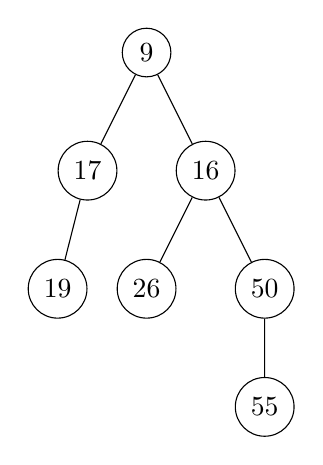
\begin{tikzpicture}
		\node[circle,draw]{9}
		child{node[circle,draw]{17}
			child{node[circle,draw,left]{19}}
		}
		child{node[circle,draw]{16}
			child{node[circle,draw]{26}}
			child{node[circle,draw]{50}
				child{node[circle,draw]{55}}
			}
		}
		;\end{tikzpicture}

	\end{center}
	
	
	\end{enumerate}	

	 \item \textbf{10.9}
	 Show how to find the second smallest value in a BinaryHeap or MeldableHeap in constant time.
	 
	 \begin{verbatim}
	 def secondSmallest(binaryHeap): 
		 
		 if binaryHeap = Empty:
			 generate ERROR  
		 else: 
			 if binaryHeap is singleton:
				 generate ERROR 
			 else:  // binary tree is not empty and greater than equal to 2
				 min(root.left,root.right) 
		 
	 
	 \end{verbatim}
	 
	 \pagebreak
	\end{enumerate}
\section*{Problem 4. Fibonacci Heap}

Solve Q19.2-1 on Page 518 in the linked reference on Fibonacci Heaps.
When going over the notes, you may skip over the theoretical discussion and assume: $\mathcal{D}(n)$ to be $log(n)$.
\begin{enumerate}
\item H.min is pointing at node 7.
	\begin{center}
	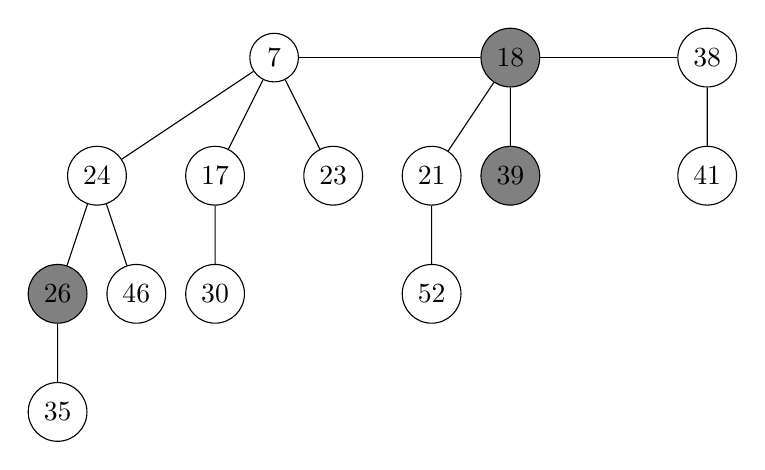
\begin{tikzpicture}
	\tikzstyle{bplus}=[rectangle split, rectangle split horizontal,rectangle split ignore empty parts,draw]
	\tikzstyle{every node}=[bplus]
	\tikzstyle{level 1}=[sibling distance=15mm]
	\tikzstyle{level 2}=[sibling distance=10mm]
	
	\node [circle, draw](a){7}
	child{node[circle,draw] {24}
		child{node[circle,draw,fill=gray] {26}
			child{node[circle,draw] {35} }}
		child{node[circle,draw] {46}}
		}
	child{node[circle,draw] {17}
		child{node[circle,draw] {30}
		}
	}
	child{node[circle,draw] {23}}
	child{node[circle,draw,fill=gray,right of=a,xshift = 20mm](b){18}
		child{node[circle,draw]{21}
		child{node[circle,draw]{52}}
			}
		child{node[circle,draw,fill=gray]{39}}
		child{node[circle,draw,right of = b,xshift = 15mm]{38}
			child{node[circle,draw]{41}}
			}
		}
	;
	\end{tikzpicture}
	\end{center}

\item  H.min is pointing to Node 18.
		\begin{center}
			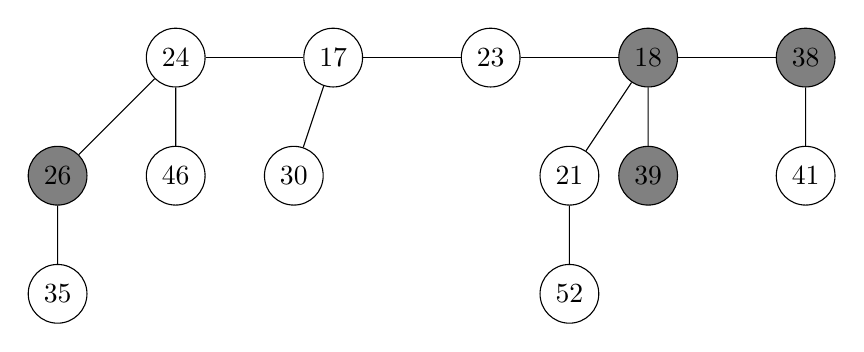
\begin{tikzpicture}
			\tikzstyle{bplus}=[rectangle split, rectangle split horizontal,rectangle split ignore empty parts,draw]
			\tikzstyle{every node}=[bplus]
			\tikzstyle{level 1}=[sibling distance=15mm]
			\tikzstyle{level 2}=[sibling distance=10mm]
			\node[circle,draw](a) {24}
			child{node[circle,draw,fill=gray] {26}
				child{node[circle,draw] {35} }}
			child{node[circle,draw] {46}}
			child{node[circle,draw,right of = a,xshift=10mm](b) {17}
				child{node[circle,draw] {30}}
				child{node[circle,draw,right of = b,xshift = 10mm](c) {23}
					child{node[circle,draw,fill=gray,right of=c,xshift = 10mm](d){18}
						child{node[circle,draw]{21}
							child{node[circle,draw]{52}}
						}
						child{node[circle,draw,fill=gray]{39}}	
						child{node[circle,draw,fill=gray,right of = d,xshift = 10mm]{38}
							child{node[circle,draw]{41}}
						}
					}
				}
			}
			;
			\end{tikzpicture}
		\end{center}

\item We create a degree array of dimension 4, because number of elements = $\log{13}$ 3rd element of array is pointing to Node 18.
\begin{tabular}{ |c|c|c|c| } 
	
	
	\hline
	nil & nil & 18 &nil \\
	\hline
	
\end{tabular}

	\begin{center}
		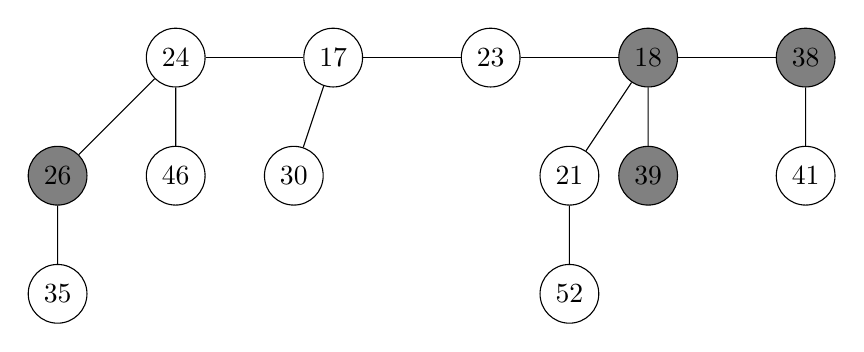
\begin{tikzpicture}
		\tikzstyle{bplus}=[rectangle split, rectangle split horizontal,rectangle split ignore empty parts,draw]
		\tikzstyle{every node}=[bplus]
		\tikzstyle{level 1}=[sibling distance=15mm]
		\tikzstyle{level 2}=[sibling distance=10mm]
		
		\node[circle,draw](a) {24}
		child{node[circle,draw,fill=gray] {26}
			child{node[circle,draw] {35} }}
		child{node[circle,draw] {46}}
		child{node[circle,draw,right of = a,xshift=10mm](b) {17}
			child{node[circle,draw] {30}}
			child{node[circle,draw,right of = b,xshift = 10mm](c) {23}
				child{node[circle,draw,fill=gray,right of=c,xshift = 10mm](d){18}
					child{node[circle,draw]{21}
						child{node[circle,draw]{52}}
					}
					child{node[circle,draw,fill=gray]{39}}	
					child{node[circle,draw,fill=gray,right of = d,xshift = 10mm]{38}
						child{node[circle,draw]{41}}
					}
				}
			}
		}
		;
		\end{tikzpicture}
	\end{center}
\item We move right from degree array, because there are no other nodes pointing to 18. Therefore, we move to the right of 18, and that is degree 1. Array[1] will not point to node 38.
\begin{tabular}{ |c|c|c|c| } 
	
	
	\hline
	nil & 38 & 18 &nil \\
	\hline
	
\end{tabular}

\begin{center}
	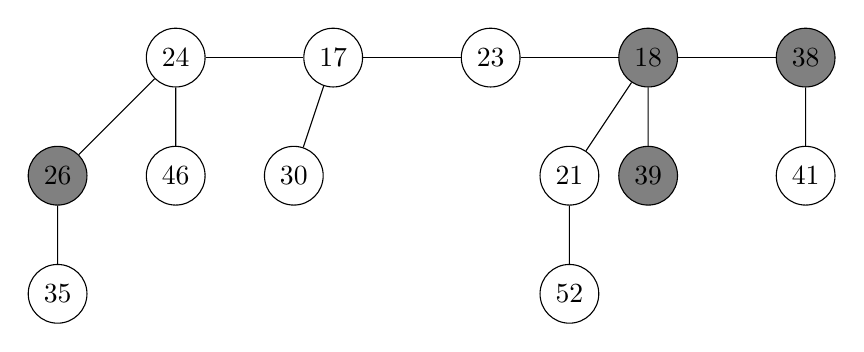
\begin{tikzpicture}
	\tikzstyle{bplus}=[rectangle split, rectangle split horizontal,rectangle split ignore empty parts,draw]
	\tikzstyle{every node}=[bplus]
	\tikzstyle{level 1}=[sibling distance=15mm]
	\tikzstyle{level 2}=[sibling distance=10mm]
	
	\node[circle,draw](a) {24}
	child{node[circle,draw,fill=gray] {26}
		child{node[circle,draw] {35} }}
	child{node[circle,draw] {46}}
	child{node[circle,draw,right of = a,xshift=10mm](b) {17}
		child{node[circle,draw] {30}}
		child{node[circle,draw,right of = b,xshift = 10mm](c) {23}
			child{node[circle,draw,fill=gray,right of=c,xshift = 10mm](d){18}
				child{node[circle,draw]{21}
					child{node[circle,draw]{52}}
				}
				child{node[circle,draw,fill=gray]{39}}	
				child{node[circle,draw,fill=gray,right of = d,xshift = 10mm]{38}
					child{node[circle,draw]{41}}
				}
			}
		}
	}
	;
	\end{tikzpicture}
\end{center}

\item We move right again. This time, a node with the same degree as degree[2] is found which was 18. We check if 26<18 and since it is not, we consolidate 18 with 26. 18 becomes parent and 26 becomes its child. 18 stays in the degree list. H.min is still pointing at 17. Since 18 now has 3 children, degree[3] is now 18, and degree[2] is changed to nil.
\begin{tabular}{ |c|c|c|c| } 
	
	
	\hline
	nil & 38 & nil & 18 \\
	\hline
	
\end{tabular}

\begin{center}
	\begin{tikzpicture}
	\tikzstyle{bplus}=[rectangle split, rectangle split horizontal,rectangle split ignore empty parts,draw]
	\tikzstyle{every node}=[bplus]
	\tikzstyle{level 1}=[sibling distance=15mm]
	\tikzstyle{level 2}=[sibling distance=10mm]
	
	\node[circle,draw,fill=gray,xshift = 10mm](a){18}
	child{node[circle,draw]{21}
		child{node[circle,draw]{52}}
	}
	child{node[circle,draw]{24}
		child{node[circle,draw,fill=gray] {26}
			child{node[circle,draw] {35} }
			}
		child{node[circle,draw] {46}}			
	}
	child{node[circle,draw,fill=gray]{39}}
		child{node[circle,draw,right of = a,xshift=20mm](b) {17}
			child{node[circle,draw] {30}}
			child{node[circle,draw,right of = b,xshift = 10mm](c) {23}
				child{node[circle,draw,fill=gray,right of = d,xshift = 10mm]{38}
					child{node[circle,draw]{41}}
				}
			}
		}
		
	;
	\end{tikzpicture}
\end{center}
\pagebreak
\item We move right again. This time, a node with the same degree as degree[1] is found which was 38. We check if 38<17 and since it is not, we consolidate 17 with 38. 17 becomes parent and 38 becomes its child. H.min is still pointing at 17. Since 17 now has two children,Array[2] becomes 17. Since 38 was marked, we unmark it after consolidate.
\begin{tabular}{ |c|c|c|c| } 	
	\hline
	nil & nil & 17 & 18 \\
	\hline
\end{tabular}

\begin{center}
	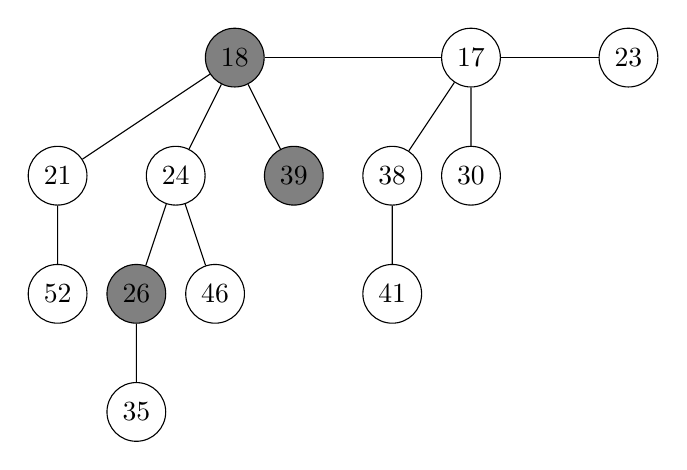
\begin{tikzpicture}
	\tikzstyle{bplus}=[rectangle split, rectangle split horizontal,rectangle split ignore empty parts,draw]
	\tikzstyle{every node}=[bplus]
	\tikzstyle{level 1}=[sibling distance=15mm]
	\tikzstyle{level 2}=[sibling distance=10mm]
	
	\node[circle,draw,fill=gray,xshift = 10mm](a){18}
	child{node[circle,draw]{21}
		child{node[circle,draw]{52}}
	}
	child{node[circle,draw]{24}
		child{node[circle,draw,fill=gray] {26}
			child{node[circle,draw] {35} }
		}
		child{node[circle,draw] {46}}			
	}
	child{node[circle,draw,fill=gray]{39}}
	child{node[circle,draw,right of = a,xshift=20mm](b) {17}
		child{node[circle,draw,](d){38}
			child{node[circle,draw]{41}}
		}
		child{node[circle,draw] {30}}
		child{node[circle,draw,right of = b,xshift = 10mm](c) {23}
		}
	}
	
	;
	\end{tikzpicture}
\end{center}
\item We move right again. There is a node of degree 0 (23), and we add it to the degree list. Since we have traversed the whole degree list, and each element's degree is unique, we return the resulting tree which is the same tree. In the next step, we look for the minimum element again, and H.min still points to 17.
\begin{tabular}{ |c|c|c|c| } 
	\hline
	23 & nil & 17 & 18 \\
	\hline
\end{tabular}

\begin{center}
	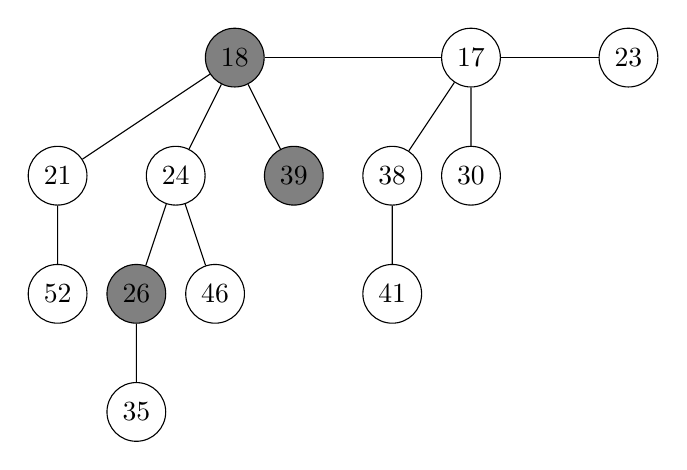
\begin{tikzpicture}
	\tikzstyle{bplus}=[rectangle split, rectangle split horizontal,rectangle split ignore empty parts,draw]
	\tikzstyle{every node}=[bplus]
	\tikzstyle{level 1}=[sibling distance=15mm]
	\tikzstyle{level 2}=[sibling distance=10mm]
	
	\node[circle,draw,fill=gray,xshift = 10mm](a){18}
	child{node[circle,draw]{21}
		child{node[circle,draw]{52}}
	}
	child{node[circle,draw]{24}
		child{node[circle,draw,fill=gray] {26}
			child{node[circle,draw] {35} }
		}
		child{node[circle,draw] {46}}			
	}
	child{node[circle,draw,fill=gray]{39}}
	child{node[circle,draw,right of = a,xshift=20mm](b) {17}
		child{node[circle,draw,](d){38}
			child{node[circle,draw]{41}}
		}
		child{node[circle,draw] {30}}
		child{node[circle,draw,right of = b,xshift = 10mm](c) {23}
		}
	}
	
	;
	\end{tikzpicture}
\end{center}
\end{enumerate}	

\end{document}
